
\documentclass[11pt]{article}
\usepackage[a4paper,landscape,left=0.45cm,right=0.45cm,top=0.45cm,bottom=0.85cm]{geometry}
\usepackage[T1]{fontenc}
\usepackage[utf8]{inputenc}
\usepackage[provide=*,french]{babel}
\usepackage{tikz}
\usepackage{graphicx}
\usepackage{eso-pic}
\usepackage{xcolor}
\usepackage{lmodern}
\usepackage{microtype}
\pagestyle{empty}
\setlength{\parindent}{0pt}

\definecolor{toporange}{RGB}{230,140,30}
\definecolor{bottomblue}{RGB}{40,97,170}
\definecolor{softgray}{RGB}{95,95,95}
\definecolor{montorange}{RGB}{255,238,220}
\definecolor{montblue}{RGB}{228,238,251}
\definecolor{brandNavy}{RGB}{11,53,112}

\newcommand{\MathsGoPrintFooter}{%
\begin{tikzpicture}[remember picture,overlay]
    \node[anchor=south west, inner sep=0pt] at ([xshift=0.42cm,yshift=0.13cm]current page.south west)
        {
\includegraphics[width=2.45cm]{../assets/img/mathsgo-logo.png}};
    \node[anchor=south, text=brandNavy!72, font=\sffamily\bfseries\fontsize{7}{7}\selectfont] at ([yshift=0.24cm]current page.south)
        {mathsgo.re \textperiodcentered\ CC BY-NC-SA 4.0};
\end{tikzpicture}%
}
\AddToShipoutPictureFG{\MathsGoPrintFooter}

\tikzset{
  writedots/.style={softgray, line width=0.9pt, line cap=round, dash pattern=on 0pt off 2.15pt}
}

% #1 = nombre d'intervalles ; #2 = labels haut ; #3 = mode libre 0/1
\newcommand{\drawPercentBoard}[3]{%
\begin{center}
\begin{tikzpicture}[x=1cm,y=1cm]
  \useasboundingbox (0,-2.65) rectangle (28.80,2.65);
  \def\xstart{5.10}
  \def\L{22.60}
  \def\ytop{1.24}
  \def\ybot{-1.32}
  \pgfmathsetmacro{\dx}{\L/(#1)}

  % Zones d'écriture
  \fill[montorange,rounded corners=5pt] (4.58,0.40) rectangle (28.10,2.08);
  \fill[montblue,rounded corners=5pt] (4.58,-2.28) rectangle (28.10,-0.36);

  % Cartouche haut : pourcentages
  \fill[montorange,rounded corners=6pt] (0.07,\ytop-1.06) rectangle (4.38,\ytop+1.02);
  \draw[toporange,line width=0.78pt,rounded corners=6pt] (0.07,\ytop-1.06) rectangle (4.38,\ytop+1.02);
  \node[font=\Large\bfseries,text=toporange] at (2.10,\ytop) {Pourcentages};

  % Cartouche bas : grandeur + unité à remplir
  \fill[montblue,rounded corners=6pt] (0.07,\ybot-1.10) rectangle (4.38,\ybot+1.06);
  \draw[bottomblue,line width=0.78pt,rounded corners=6pt] (0.07,\ybot-1.10) rectangle (4.38,\ybot+1.06);
  \node[anchor=west,font=\large\bfseries,text=bottomblue] at (0.35,\ybot+0.60) {Grandeur :};
  \draw[writedots] (0.35,\ybot-0.18)--(4.02,\ybot-0.18);
  \node[anchor=west,font=\large\bfseries,text=bottomblue] at (0.35,\ybot-0.66) {Unité :};
  \draw[writedots] (2.20,\ybot-0.84)--(4.02,\ybot-0.84);

  % Lignes principales
  \draw[toporange,line width=1.45pt,-stealth] (\xstart,\ytop)--(\xstart+\L+0.32,\ytop);
  \draw[bottomblue,line width=1.45pt,-stealth] (\xstart,\ybot)--(\xstart+\L+0.32,\ybot);

  % Graduations + pointillés de la ligne du bas
  \foreach \i in {0,...,#1}{
    \pgfmathsetmacro{\x}{\xstart + \i*\dx}
    \draw[toporange,line width=0.82pt] (\x,\ytop-0.15)--(\x,\ytop+0.15);
    \draw[bottomblue,line width=0.82pt] (\x,\ybot-0.15)--(\x,\ybot+0.15);
    \draw[writedots] (\x-0.35,\ybot-0.84)--(\x+0.35,\ybot-0.84);
  }

  % Labels haut
  \ifnum#3=0
    \foreach \i/\lab in {#2}{
      \pgfmathsetmacro{\x}{\xstart + \i*\dx}
      \node[font=\bfseries\large,text=toporange] at (\x,\ytop+0.45) {\lab};
    }
  \else
    \foreach \i in {0,...,#1}{
      \pgfmathsetmacro{\x}{\xstart + \i*\dx}
      \draw[writedots] (\x-0.35,\ytop+0.45)--(\x+0.35,\ytop+0.45);
    }
  \fi
\end{tikzpicture}
\end{center}
}

\newcommand{\titreCompact}{%
\begin{center}
  {\LARGE\bfseries\textcolor{brandNavy}{Pourcentages — double ligne graduée}}
\end{center}
}

\begin{document}

% Page 1 : deux gabarits mieux répartis sur la page
\titreCompact
\vspace*{0.05cm}
\vfill
\drawPercentBoard{4}{0/0\%,1/25\%,2/50\%,3/75\%,4/100\%}{0}
\vfill
\drawPercentBoard{10}{0/0\%,1/10\%,2/20\%,3/30\%,4/40\%,5/50\%,6/60\%,7/70\%,8/80\%,9/90\%,10/100\%}{0}
\vfill

\newpage

% Page 3 : gabarit gradué au 1 %, seul sur la page
\titreCompact
\vspace*{0.18cm}
\vfill

\begin{center}
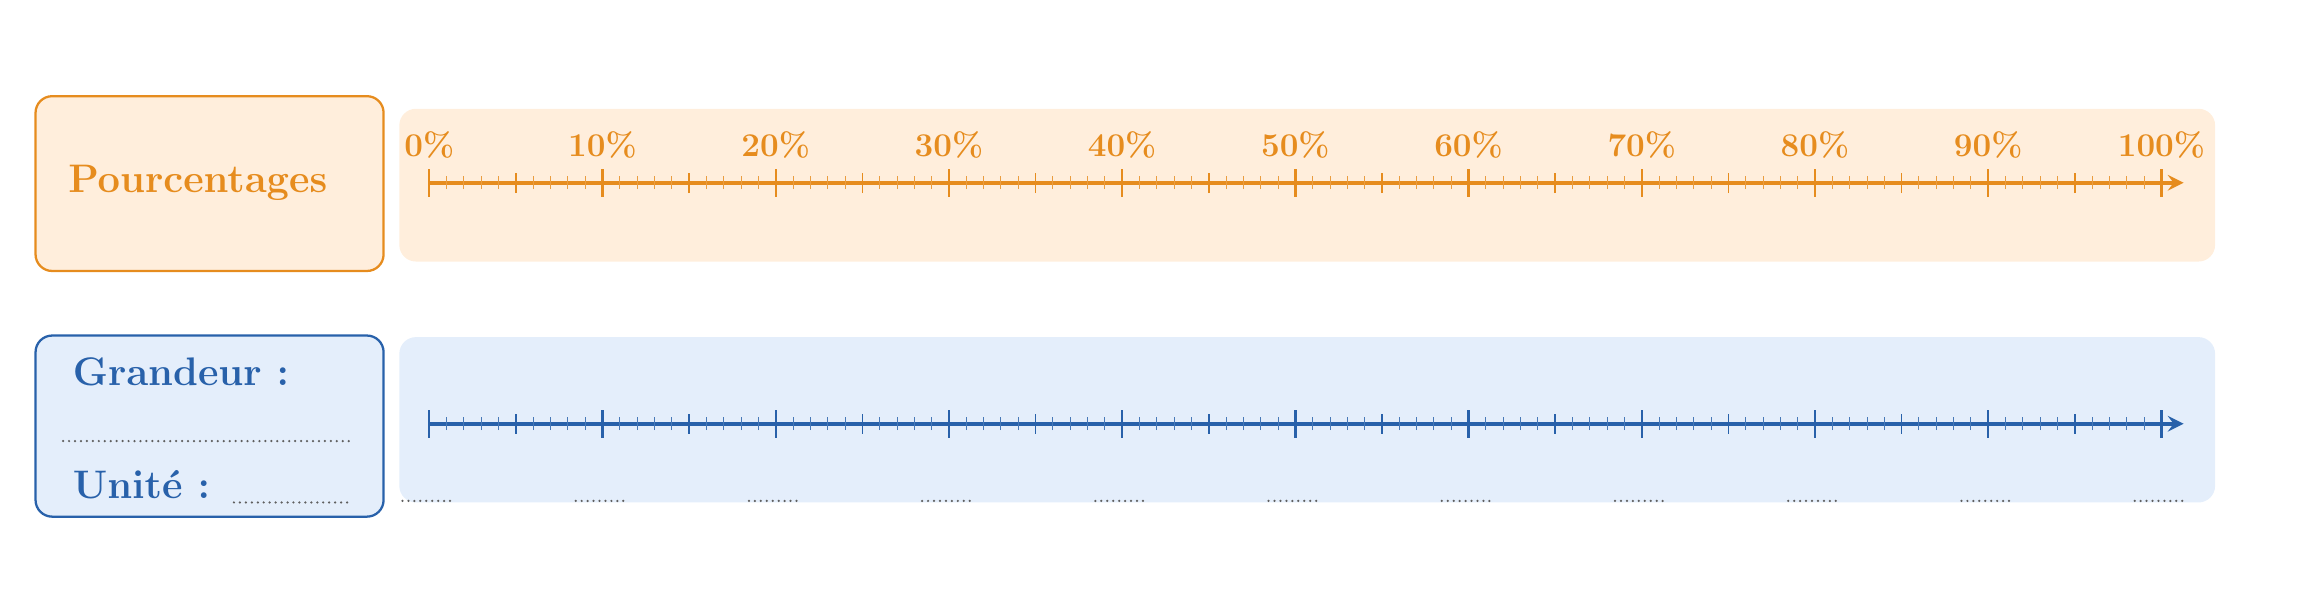
\begin{tikzpicture}[x=1cm,y=1cm]
  \useasboundingbox (0,-3.45) rectangle (28.60,3.45);
  \def\xstart{5.10}
  \def\L{22.00}
  \def\ytop{1.48}
  \def\ybot{-1.58}

  % zones d'écriture
  \fill[montorange,rounded corners=6pt] (4.72,0.48) rectangle (27.78,2.42);
  \fill[montblue,rounded corners=6pt] (4.72,-2.58) rectangle (27.78,-0.48);

  % cartouches
  \fill[montorange,rounded corners=6pt] (0.10,\ytop-1.12) rectangle (4.52,\ytop+1.10);
  \draw[toporange,line width=0.82pt,rounded corners=6pt] (0.10,\ytop-1.12) rectangle (4.52,\ytop+1.10);
  \node[font=\Large\bfseries,text=toporange] at (2.16,\ytop) {Pourcentages};

  \fill[montblue,rounded corners=6pt] (0.10,\ybot-1.18) rectangle (4.52,\ybot+1.12);
  \draw[bottomblue,line width=0.82pt,rounded corners=6pt] (0.10,\ybot-1.18) rectangle (4.52,\ybot+1.12);
  \node[anchor=west,font=\Large\bfseries,text=bottomblue] at (0.45,\ybot+0.66) {Grandeur :};
  \draw[writedots] (0.45,\ybot-0.22)--(4.10,\ybot-0.22);
  \node[anchor=west,font=\Large\bfseries,text=bottomblue] at (0.45,\ybot-0.78) {Unité :};
  \draw[writedots] (2.62,\ybot-1.00)--(4.10,\ybot-1.00);

  % lignes principales
  \draw[toporange,line width=1.48pt,-stealth] (\xstart,\ytop)--(\xstart+\L+0.28,\ytop);
  \draw[bottomblue,line width=1.48pt,-stealth] (\xstart,\ybot)--(\xstart+\L+0.28,\ybot);

  % graduations : 1 % avec repères plus marqués tous les 10 %
  \foreach \i in {0,...,100}{
    \pgfmathsetmacro{\x}{\xstart + \i*(\L/100)}
    \ifnum\i=0
      \draw[toporange,line width=0.84pt] (\x,\ytop-0.18)--(\x,\ytop+0.18);
      \draw[bottomblue,line width=0.84pt] (\x,\ybot-0.18)--(\x,\ybot+0.18);
    \else\ifnum\i=100
      \draw[toporange,line width=0.84pt] (\x,\ytop-0.18)--(\x,\ytop+0.18);
      \draw[bottomblue,line width=0.84pt] (\x,\ybot-0.18)--(\x,\ybot+0.18);
    \else
      \pgfmathtruncatemacro{\modten}{mod(\i,10)}
      \pgfmathtruncatemacro{\modfive}{mod(\i,5)}
      \ifnum\modten=0
        \draw[toporange,line width=0.84pt] (\x,\ytop-0.18)--(\x,\ytop+0.18);
        \draw[bottomblue,line width=0.84pt] (\x,\ybot-0.18)--(\x,\ybot+0.18);
      \else\ifnum\modfive=0
        \draw[toporange,line width=0.55pt] (\x,\ytop-0.13)--(\x,\ytop+0.13);
        \draw[bottomblue,line width=0.55pt] (\x,\ybot-0.13)--(\x,\ybot+0.13);
      \else
        \draw[toporange!85,line width=0.32pt] (\x,\ytop-0.08)--(\x,\ytop+0.08);
        \draw[bottomblue!85,line width=0.32pt] (\x,\ybot-0.08)--(\x,\ybot+0.08);
      \fi\fi
    \fi\fi
  }

  % repères de pourcentage tous les 10 %
  \foreach \i in {0,10,...,100}{
    \pgfmathsetmacro{\x}{\xstart + \i*(\L/100)}
    \node[font=\bfseries\large,text=toporange] at (\x,\ytop+0.48) {\i\%};
    \draw[writedots] (\x-0.34,\ybot-0.98)--(\x+0.34,\ybot-0.98);
  }
\end{tikzpicture}
\end{center}

\vfill

\end{document}
